\newglossaryentry{Charles D. Moore}
{
  name={Charles D. Moore},
  description={Charles D. Moore, is the inventor of the forth programming language.}
}

\chapter{Results}
\label{chap:Results}

In this chapter, I will introduce the chosen Forth software system. Afterwards, I will present the manually or semi automatically produced graphics according to the selected visualization methods.

\section{The software under investigation: Brainless}

Brainless\footnote{Brainless verion 0.1.2 is used, the source code can be optained on \url{http://sourceforge.net/projects/forth-brainless/}} is a chess-playing program written in ANS Forth. The source code consists of several files with an overall size\footnote{The command to calculate the size was \emph{find . -name '*.fs' -maxdepth 1 | xargs wc -l}} of 139497 bytes and 4108 lines of code\footnote{The command used to count the lines of code, was \emph{find . -name '*.fs' -maxdepth 1 | xargs wc -l}}.
This measure is somehow controversial, but since the files contain only a short header and are formatted in the usual manner, it seems appropriate for comparison. The code is organized in a flat structure. There is one directory with 30 files, which contain 663 words. There is only one custom word list defined. Thus the visualization of a word list hierarchy makes obviously little sense and is left out in the following sections.

The other software system, I took into consideration, was brew\footnote{brew version 0.2.0 was used. The source code can be obtained on \url{http://www.robertepprecht.ch/brew/index.html}}. Brew is a 'playground for evolutionary programming', as the author calls it. Due to its size of 1062857 bytes and 36801 lines of code, this project seemed too large to be analyze manually in reasonable time.

For the following figures, I used a snapshot of an execution trace.
Since the calculations of the computer-moves produce a huge amount of word executions, the example trace, was created by making only the player-move: \emph{d2 d3 m} \keys{\return}. The snapshot contains all word executions after and including the execution of the word \emph{m}. It consists of 4709 word executions. \ref{fig:brainless_before_m} and \ref{fig:brainless_after_m} show the state of the game before and after entering \emph{d2 d3 m} \keys{\return}.

\begin{figure}[p]
    \centering
    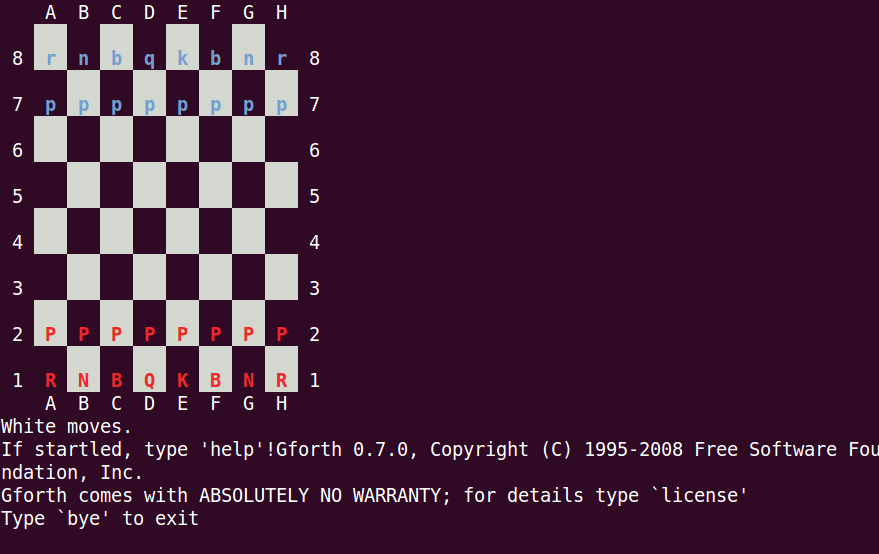
\includegraphics[scale=0.4]{graphics/brainless_before.png}
    \caption{State of the game before entering \emph{d2 d3 m}}
    \label{fig:brainless_before_m}
\end{figure}

\begin{figure}[p]
    \centering
    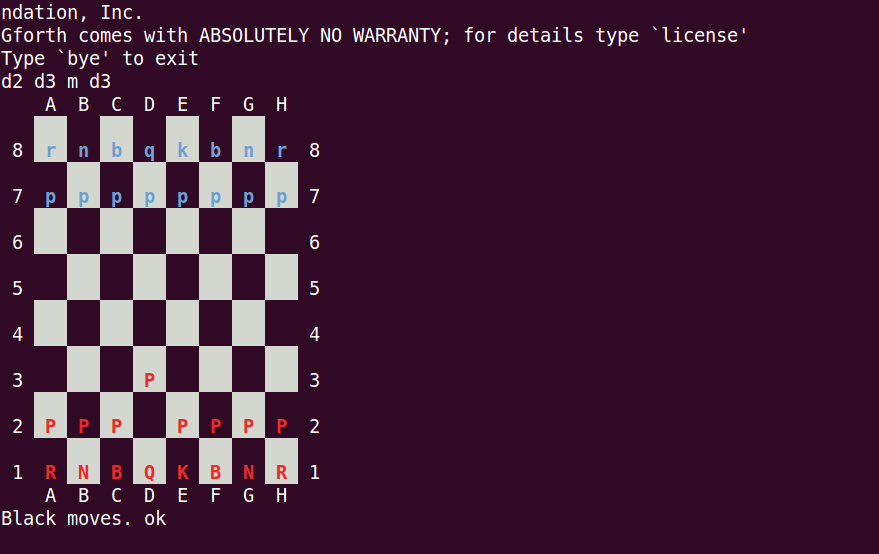
\includegraphics[scale=0.4]{graphics/brainless_after.png}
    \caption{State of the game after entering \emph{d2 d3 m}}
    \label{fig:brainless_after_m}
\end{figure}

\section{The application of the previously presented methods}

\subsection*{Hierarchical edge bundles}

Figure \ref{fig:hierarchic_edge_bundle} shows the first 100\footnote{The calculation of the interaction lines consume a considerable amount of system resources, which prevents longer traces due to memory limitation.} word executions of the trace snapshot mentioned before in a \emph{hierarchic edge bundle}.

The outer ring labeled with \emph{brainless-0.1.2} represents the directory of the source code, the middle ring represents the files and the inner ring represents the words. Words which haven't been executed in this snapshot, have been omitted.
The word sectors are of equal angle, the number of different words divided by 360\degree. The file sectors' angle have been adjusted according to the number of files they contain.
The lines in the circle represent word executions. Same as in \cite{Holten:2006:HEB:1187627.1187772}, the word on the green end is the caller and the word on the red end is the callee. The distance of the turning point to the center of the circle depends on the distance(in degree) of the two word sectors, words with great distance are connected near to center. Multiple occurrences of caller/callee pair appear as one line in this graph. The exact algorithms used to calculate \ref{fig:hierarchic_edge_bundle} can be found in \hl{<appendix>}.

\subsubsection*{Interpretation}
The main problem in this manually generated picture is the limitation to  100 executions. Due to rendering time and memory requirement, it was not possible to visualize more executions with KTikZ\footnote{Version 0.10}.
Apart from that, the hierarchic edge bundle provides information on the complexity or importance of a word in this part of the execution trace(the number of words which are executed by one word, the number of distinct words which are executed by one word or the number of words which call on word).
Provided, that words are named expressively, the hierarchic edge bundle can also help to extract information on what happened during execution and how something happened.

\subsubsection*{Possible improvements}
A further improvement would be to draw multiple occurrences of the same caller/callee pairs(the interaction lines) with a slight gap to visualize all the executions. Or, if there are too many interaction lines, to show the exact number of interactions(e.g. on hover).
Another improvement would be to show the name of the words in the hierarchic part, or if there are too much, to show it on hover.
Due to the limitation to 100 executions, the not involved words could be omitted in the hierarchic part.

\begin{figure}[p]
    \centering
    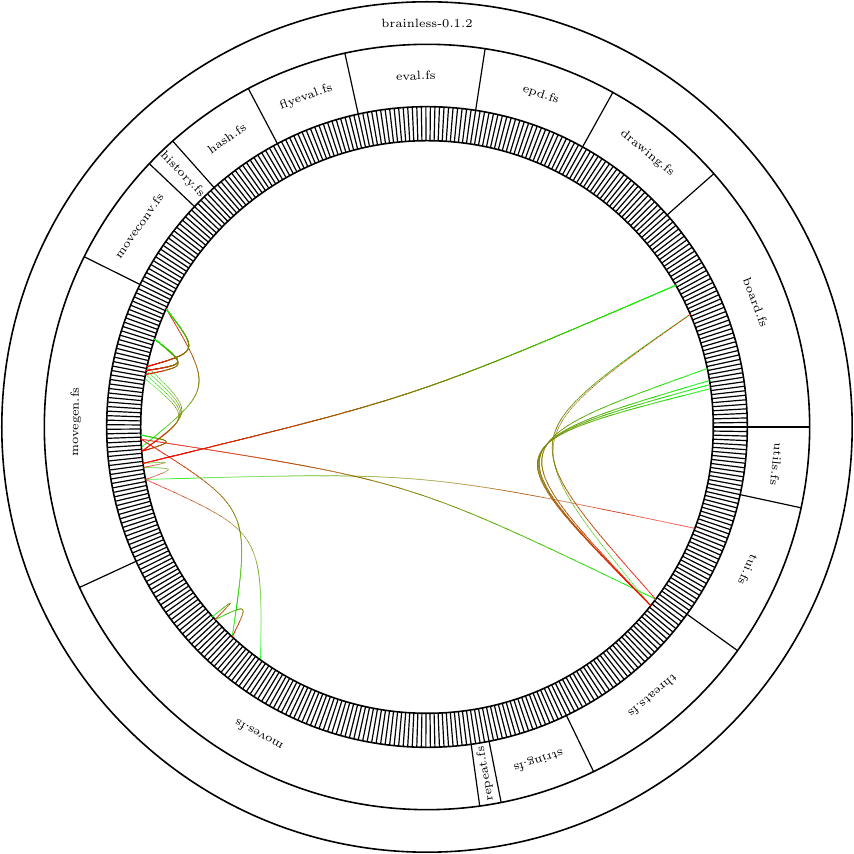
\includegraphics[scale=0.65]{graphics/hierarchic_edge_bundle-dir_file_word.png}
    \caption{Hierarchic edge bundle of a small snapshot of the trace of Brainless after \emph{d2 d3 m}}
    \label{fig:hierarchic_edge_bundle}
\end{figure}


\subsection*{Information murals and massive sequence view}

Figures \ref{fig:massive_sequence_view_1}, \ref{fig:massive_sequence_view_2} and \ref{fig:massive_sequence_view_3} show the trace snapshot in a \emph{massive sequence view}.

The \emph{massive sequence view} consists of a hierarchical part at the top of \ref{fig:massive_sequence_view_1} and the interaction part which follows immediately(\ref{fig:massive_sequence_view_2} and \ref{fig:massive_sequence_view_3}). The upper level of the hierarchical part labeled with \emph{brainless-0.1.2}, again, represents the directory of the source code. The middle level, the files and the lower level, the words. Again, words which haven't been executed in this snapshot, have been omitted.
The interaction part shows the word executions as lines. As in \cite{Holten:2006:HEB:1187627.1187772}, the word above the green end is the caller and the word above the red end is the callee. The order of the interaction lines represents also the order of execution. The first executed word is represented by the upper most interaction line.

\subsubsection*{Interpretation}

It is easy to identify certain steps of the program execution like the drawing part at the end of the trace(interaction with drawing.fs shown if figure \ref{fig:massive_sequence_view_2}) and the file writing part(interaction from epd.fs at the and of figure \ref{fig:massive_sequence_view_2}), if one know the words contained in those files.

\subsubsection*{Possible improvements}

\ref{fig:massive_sequence_view_1}, \ref{fig:massive_sequence_view_2} and \ref{fig:massive_sequence_view_3} clearly show the lack of interactivity. Without filtering, zooming, on-demand information on words(references to source code) and of course expressive naming, it still remains hard to map the sections of the trace to behavior. Besides these concerns, the massive sequence view seems to be well applicable to forth program traces.

\begin{figure}[p]
    \centering
    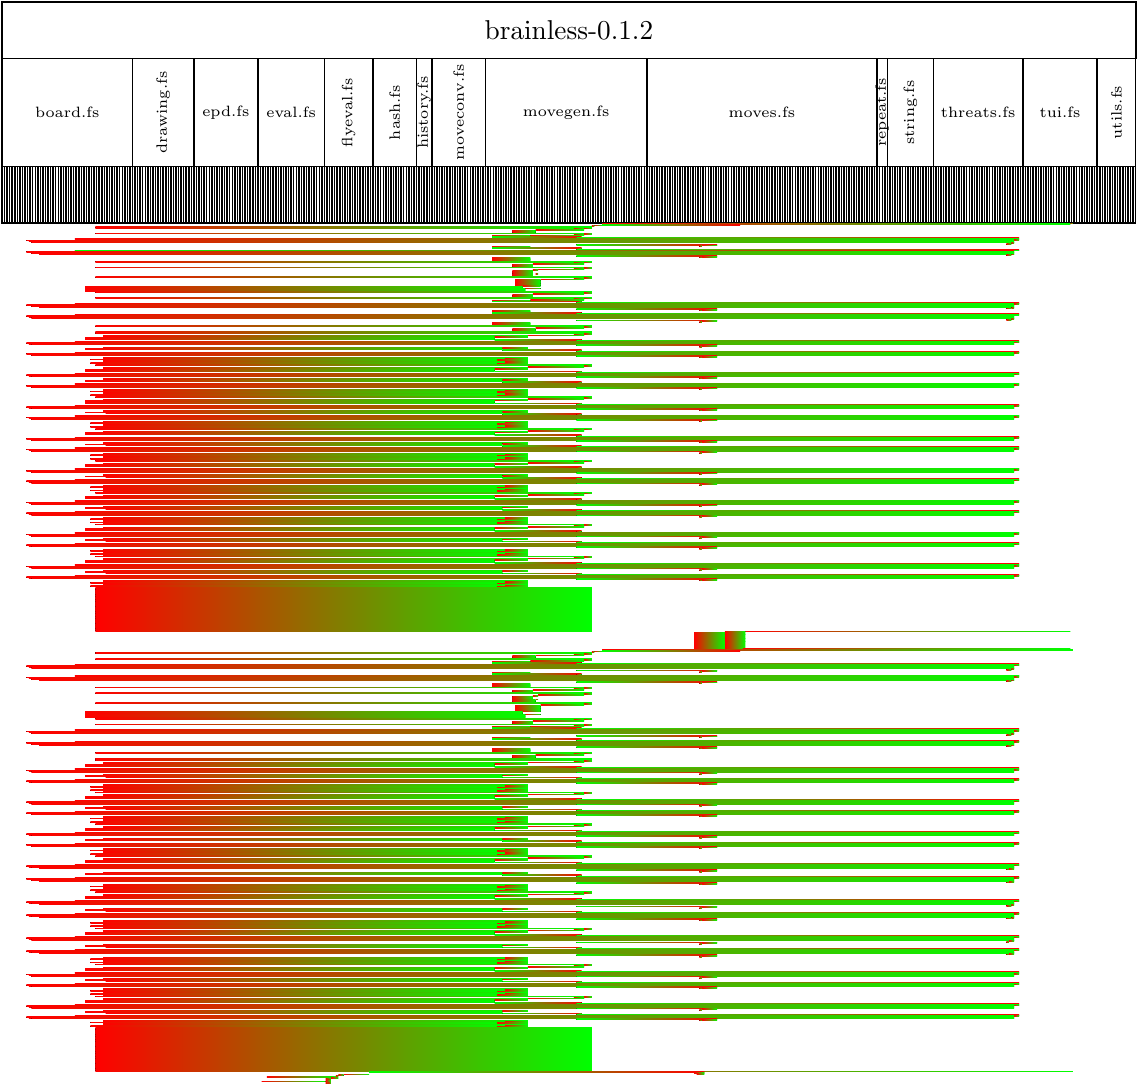
\includegraphics[scale=0.52]{graphics/massive_sequence_view-dir_file_word_1.png}
    \caption{Massive sequence view(Part 1) of Brainless after \emph{d2 d3 m}}
    \label{fig:massive_sequence_view_1}
\end{figure}

\begin{figure}[p]
    \centering
    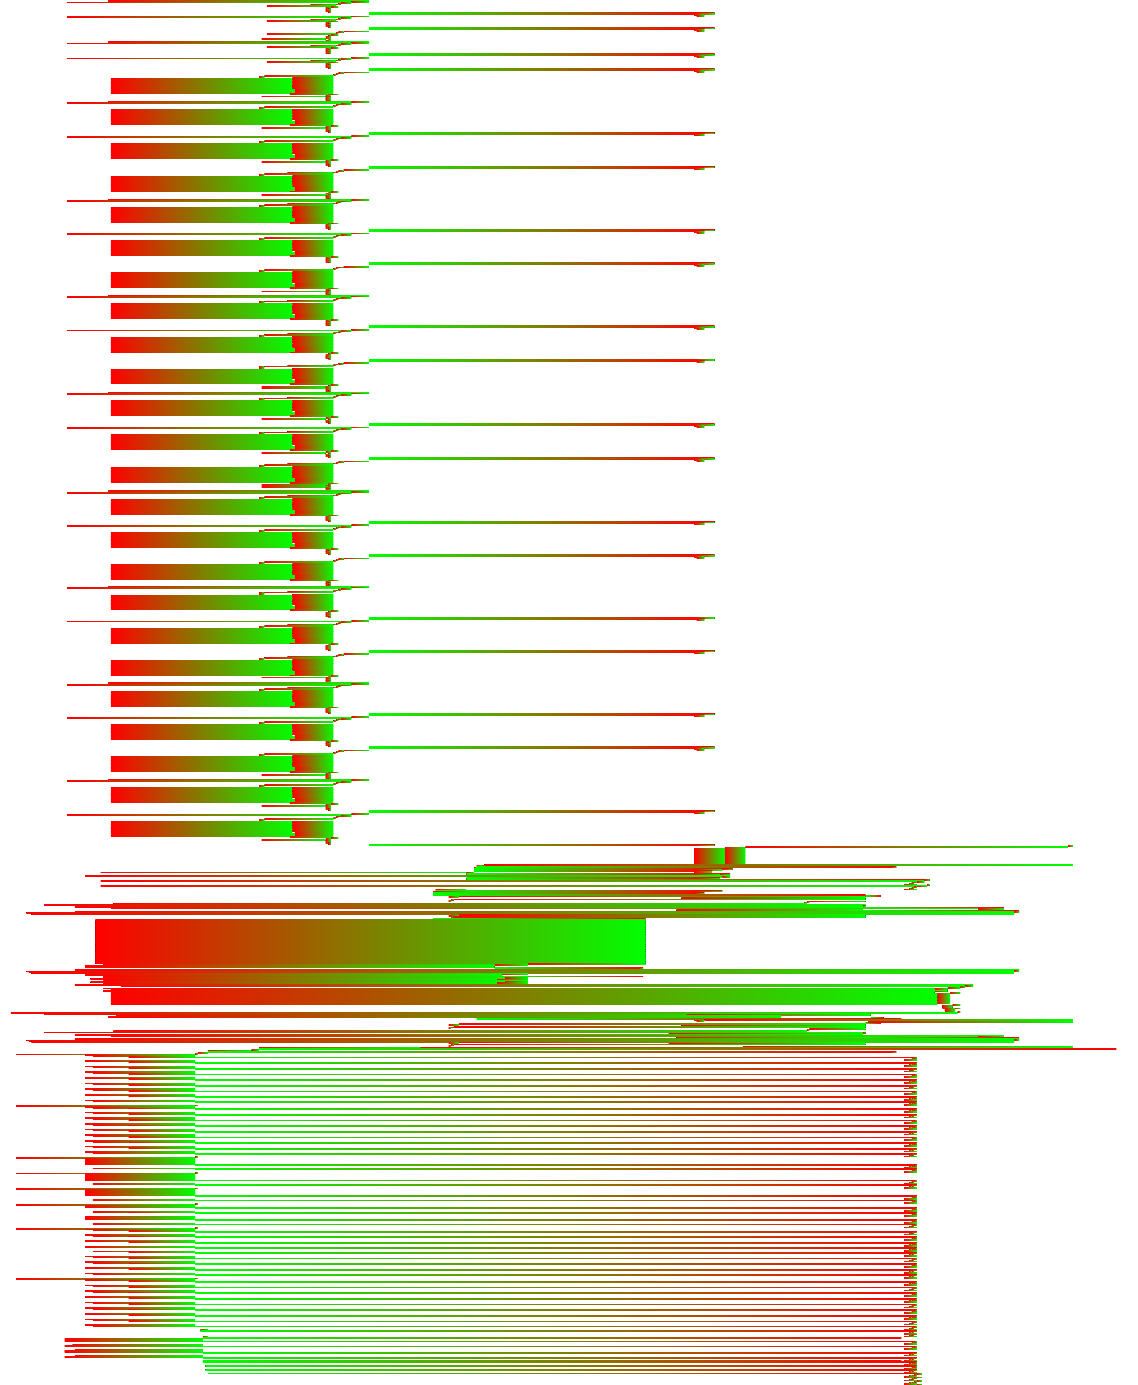
\includegraphics[scale=0.52]{graphics/massive_sequence_view-dir_file_word_2.png}
    \caption{Massive sequence view(Part 2) of Brainless after \emph{d2 d3 m}}
    \label{fig:massive_sequence_view_2}
\end{figure}

\begin{figure}[p]
    \centering
    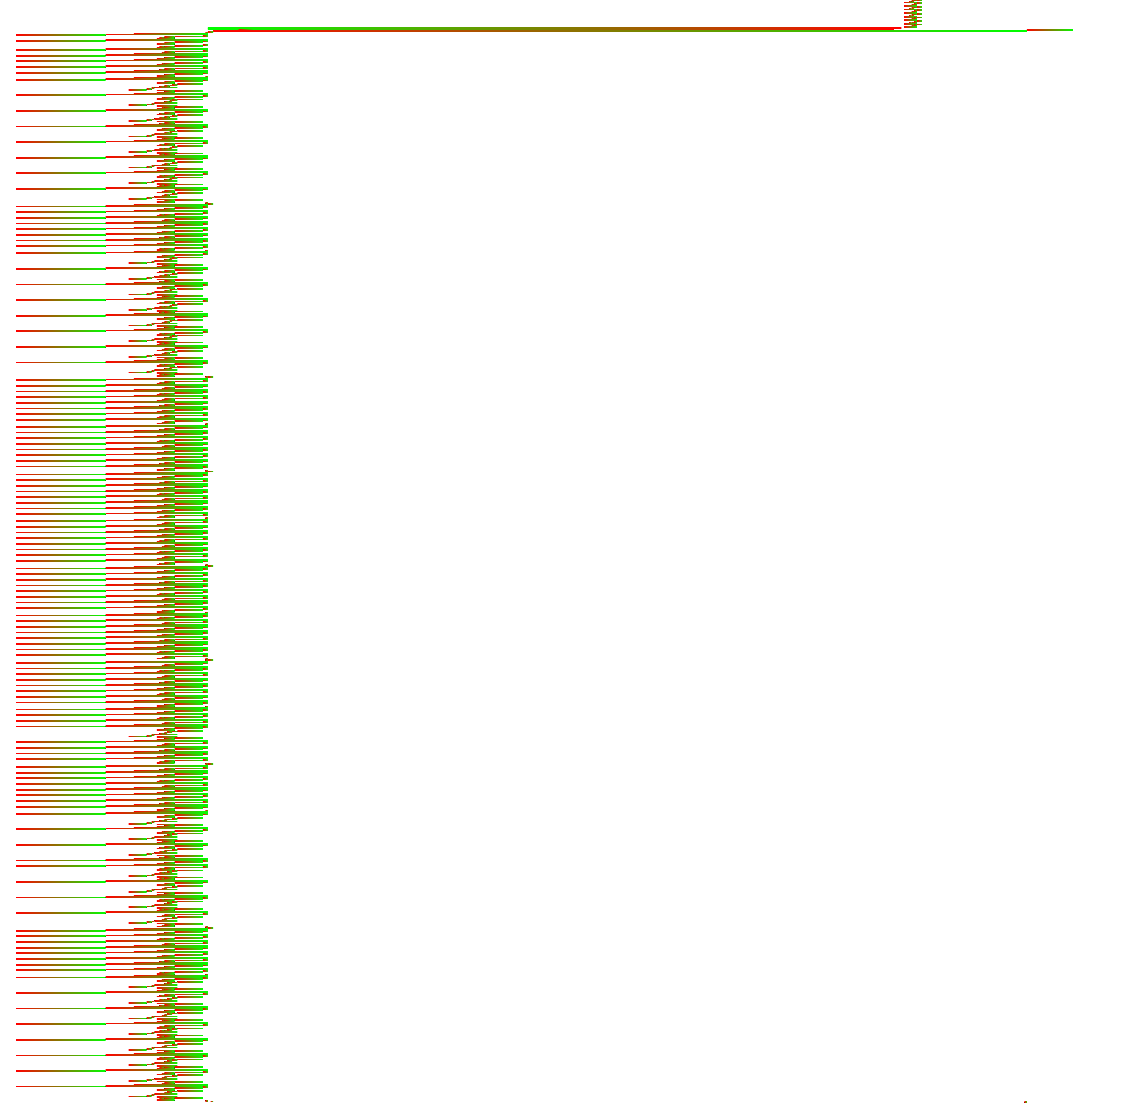
\includegraphics[scale=0.52]{graphics/massive_sequence_view-dir_file_word_3.png}
    \caption{Massive sequence view(Part 3) of Brainless after \emph{d2 d3 m}}
    \label{fig:massive_sequence_view_3}
\end{figure}

\subsection*{High-Level polymetric views}

Figure \ref{fig:polymetric_view} shows a polymetric view of the snapshot. 
I used a circle to represent a single word. The radius reflects the number of executions, frequently executed words appear as larger circles. The position(distance from the origin) reflects the number of words executed within the word, fewer sub-word-executions result in a greater distance. If the number of sub executions vary, the maximum was used. The color of a circle reflects the io-behavior of a word. Red means, the word prints to stdout and yellow means it is reading from or writing to a file.

\subsubsection*{Interpretation}

<TODO Red big circle> \ref{fig:polymetric_view_detail}

\subsubsection*{Possible improvements}

\hl{TODO gro�e w�rter = performance relevant, w�rter die in der mitte sind, sind eher intern komplex, farben: w�rter die tats�chlich was sichtbares tun}

\begin{figure}[p]
    \centering
    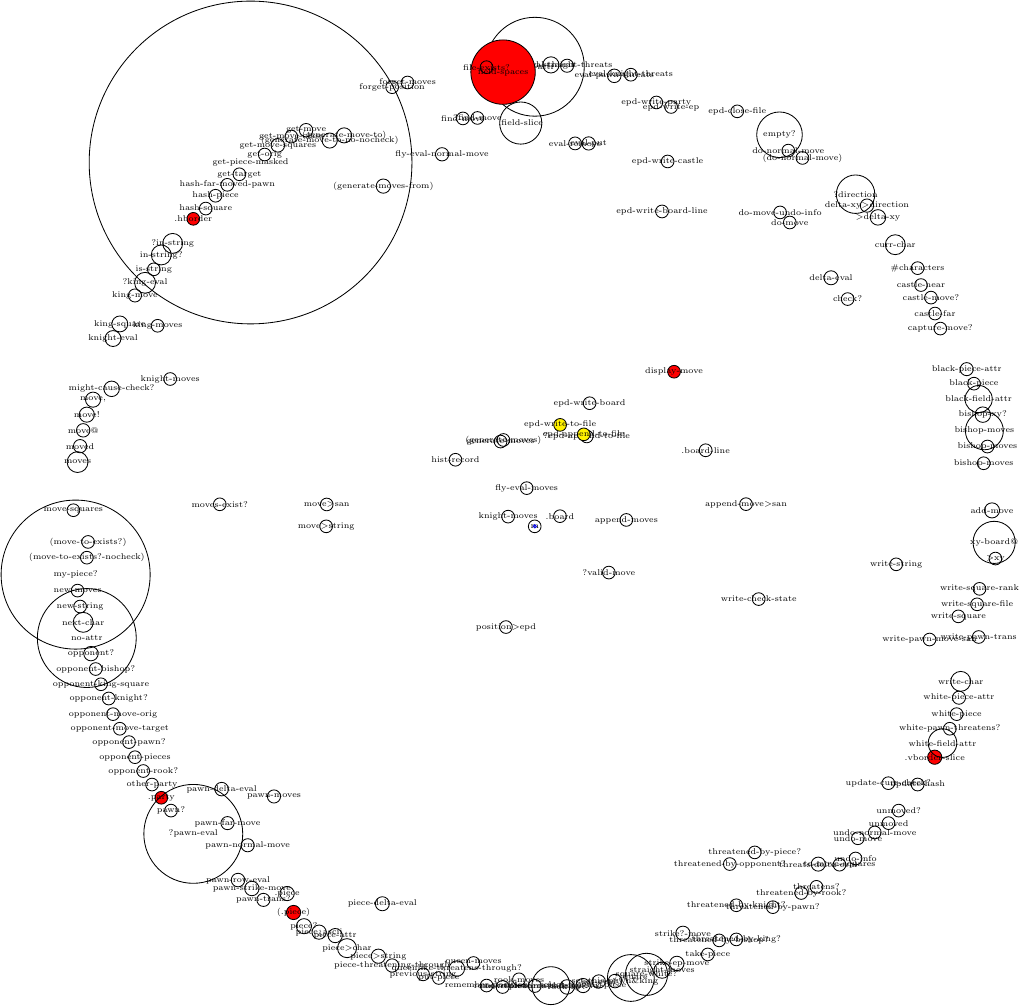
\includegraphics[scale=0.55]{graphics/polymetric_view.png}
    \caption{High-Level polymetric view of the trace of Brainless after \emph{d2 d3 m}}
    \label{fig:polymetric_view}
\end{figure}

\begin{figure}[p]
    \centering
    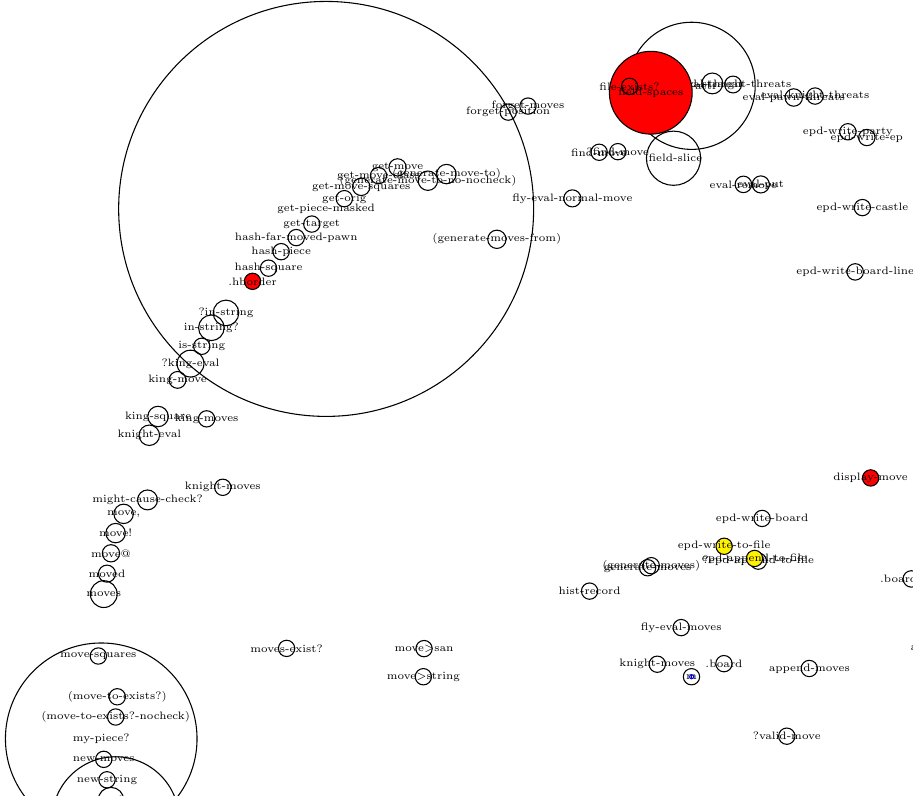
\includegraphics[scale=0.5]{graphics/polymetric_view_detail.png}
    \caption{Sanpshot of the polymetric view of the trace of Brainless after \emph{d2 d3 m}}
    \label{fig:polymetric_view_detail}
\end{figure}

\subsection*{Memory access view}

Figure \ref{fig:taxonomy} shows a small snapshot of the memory access of brainless.
It shows the words and the memory locations they access. The words are represented by circles and the memory locations(values) by rectangles. The arrows represent the direction of the access. An outgoing arrow(from a word to a memory location) represents write operation and an incoming arrow(from a memory location to a word), a read operation.
Since Brainless makes extensive use of \emph{value}s, does not use *\emph{variable}s at all and uses custom defining words only occasionally, \ref{fig:taxonomy} shows only the \emph{value}s.

\subsubsection*{Interpretation}

\subsubsection*{Possible improvements}

It should cover \emph{value}, \emph{variable}, \emph{2variable}, \emph{fvariable} and also memory fields, allocated by custom defining words.

\begin{figure}[p]
    \centering
    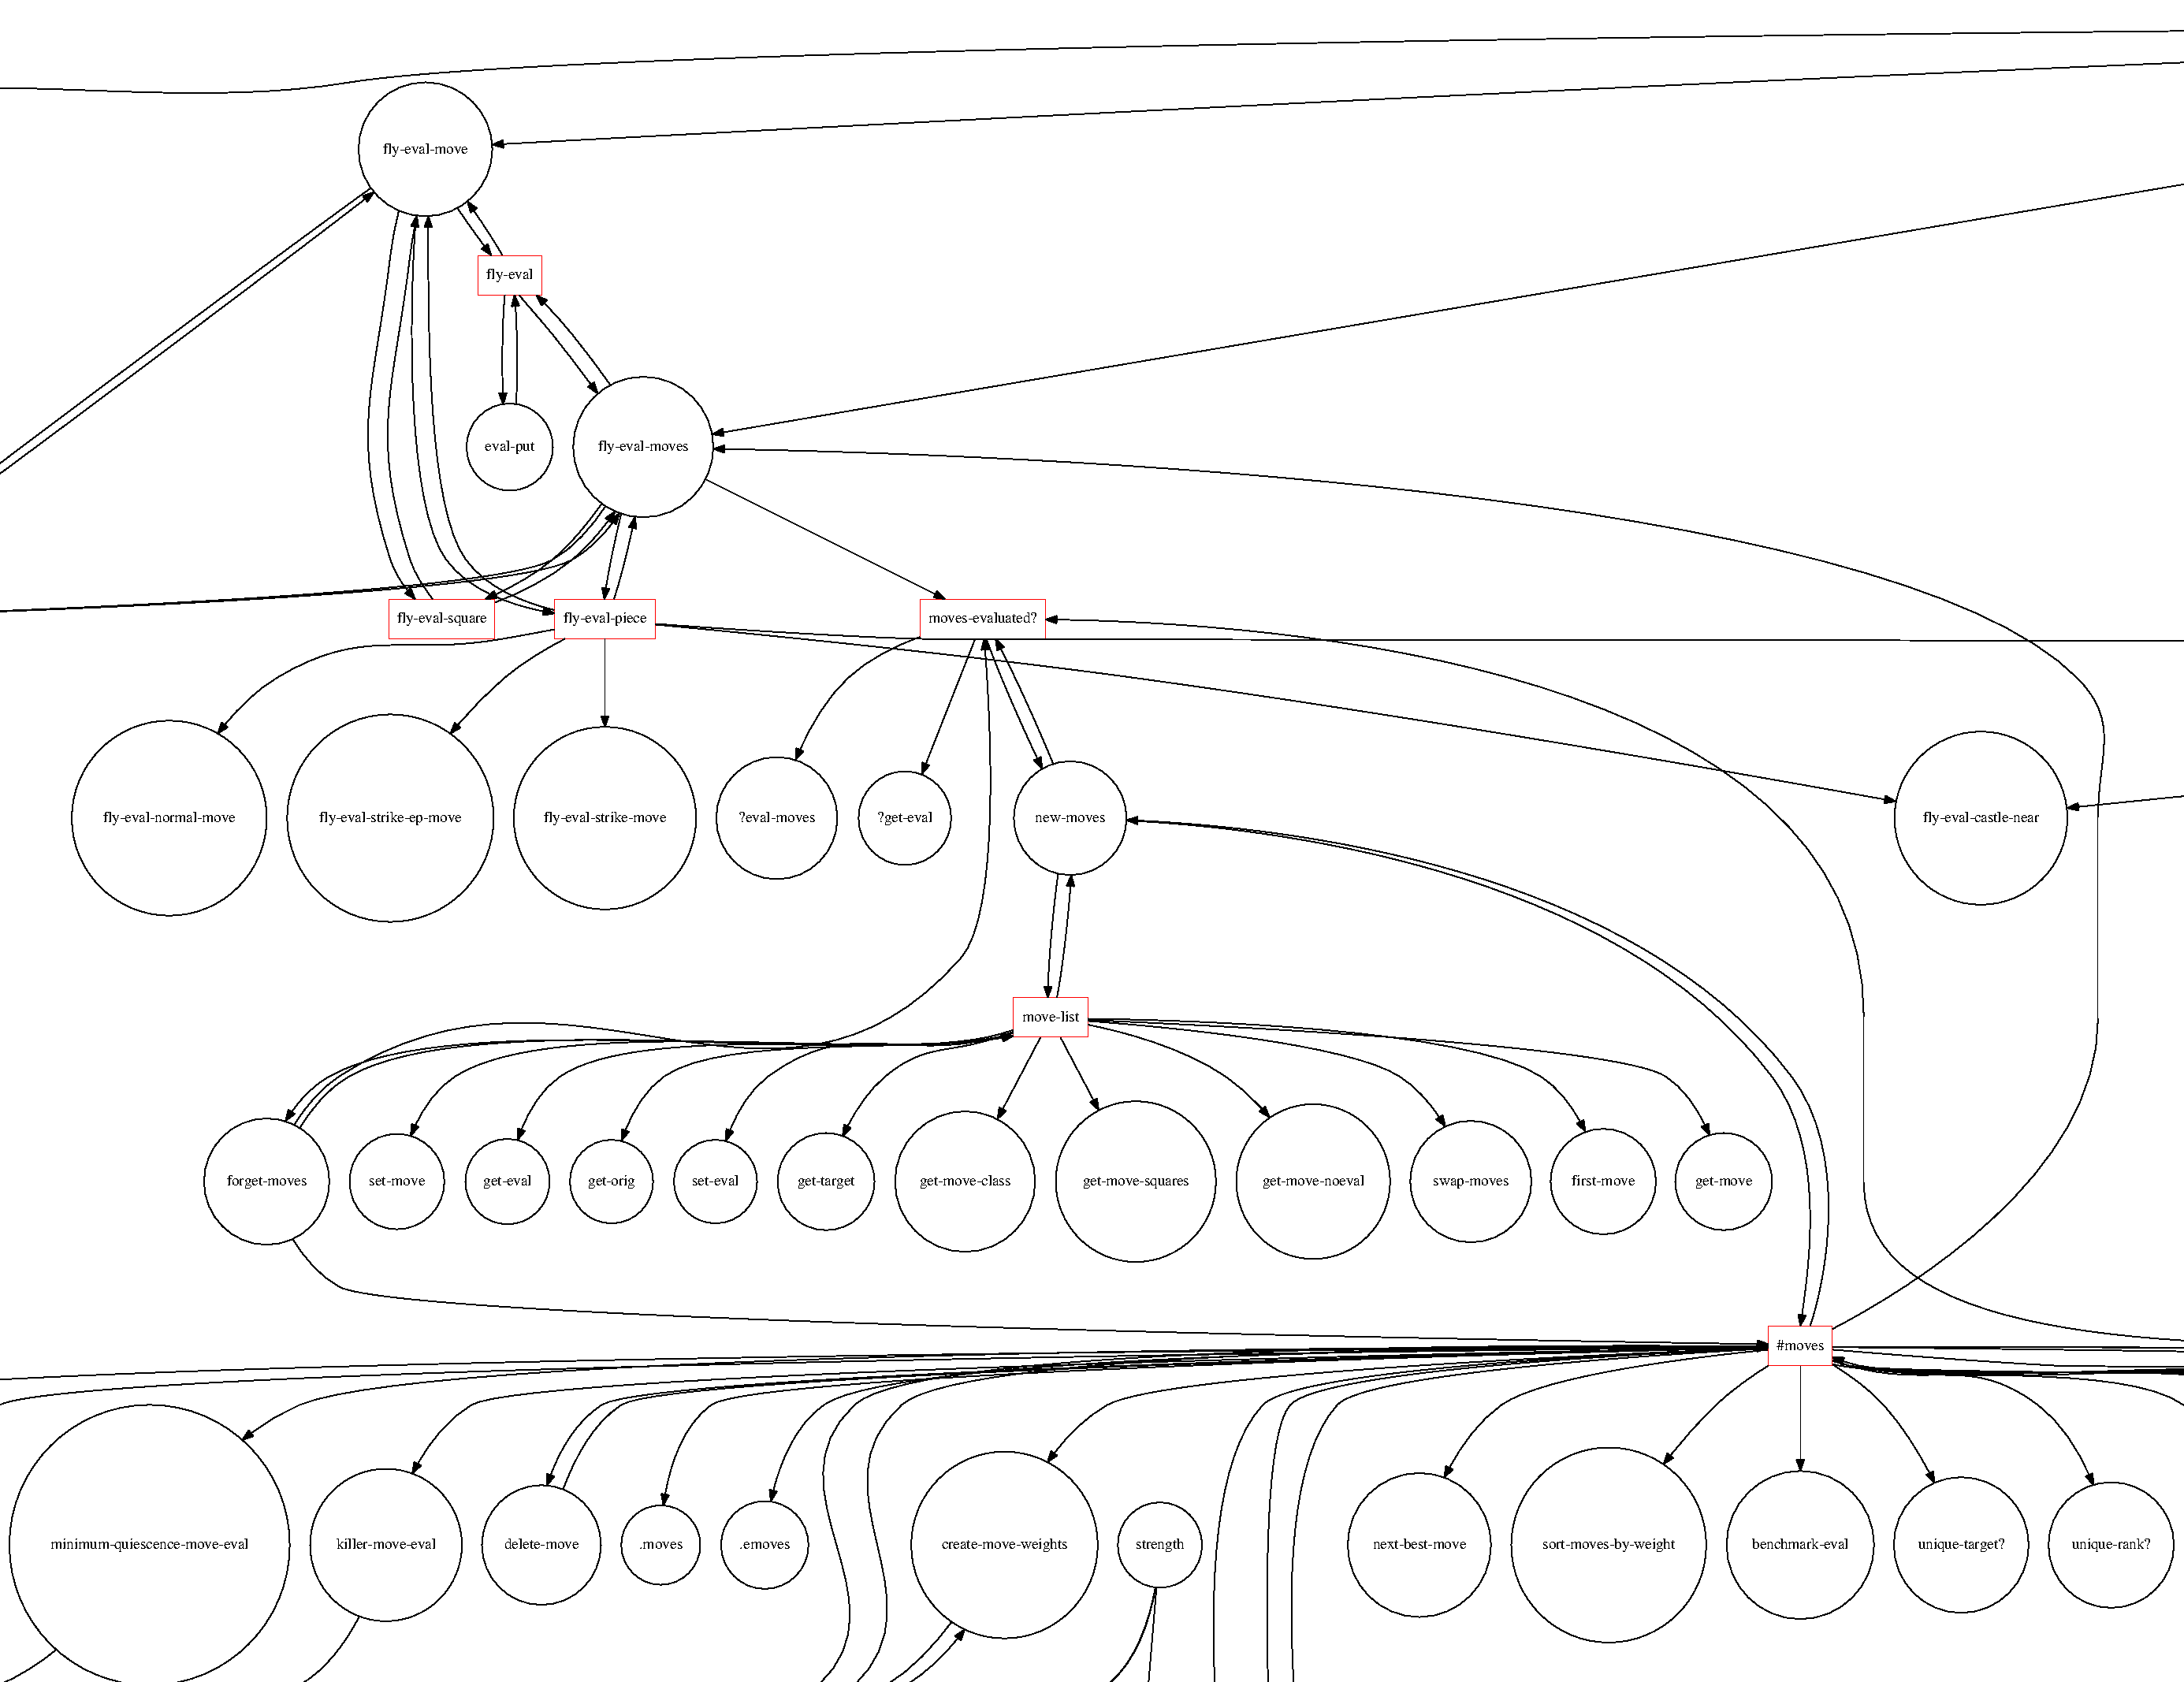
\includegraphics[scale=0.20]{graphics/taxonomy_view2.png}
    \caption{Snapshot of the memory access of Brainless}
    \label{fig:taxonomy}
\end{figure}

\section{gfvis - A trace visualization enhancement for Gforth}

Gfvis was developed within this thesis, it is an enhancement for Gforths debugger \emph{dbg}\ref{chap:StateOfTheArt}.
Gfvis runs with a slightly modified version of Gforth(gforth-itc) and requires \emph{gv}\footnote{GV is a postscript viewer for X displays. For further information see: \url{http://www.gnu.org/software/gv/}}. It consist of \emph{gfvis.fs} and \emph{gfvis.ps}. Both have to be in the same directory. \emph{gfvis.ps} is a template file, written in postscript, it contains code to display the executed words and the state of the data stack, the floating stack and the return stack. \emph{gfvis.fs} contains code which collects the information to be displayed and to create and update \emph{trace.fs}.
\\
Gfvis is started by executing \verb|<path to modified gforth>/gforth-itc ./gfvis.fs|. When the dbg is started(i.e.\ \verb|dbg test|), trace.ps, a copy of gfvis.ps, is created and gv is started to display its content \ref{fig:traceps1}\ref{fig:traceps2}. From then on, every executed word, updates trace.ps with the name of the word and the state of the stacks. When \verb|bye| is executed, gfvis terminates gv and gforth-itc.

\subsubsection*{Interpretation}

\subsubsection*{Possible improvements}

Inefficient use of space, on demand display of stack content.
\begin{itemize}
\item display content of value, variable and custom defined memory
\item display of allocated memory areas and tracking changes in those
\item better visualization of the stacks and of changes of stack elements
\item better visualization of loops and control structures
\item using a standard data type to store traces
\item limited stack depth per word
\end{itemize}


\begin{figure}[p]
    \centering
    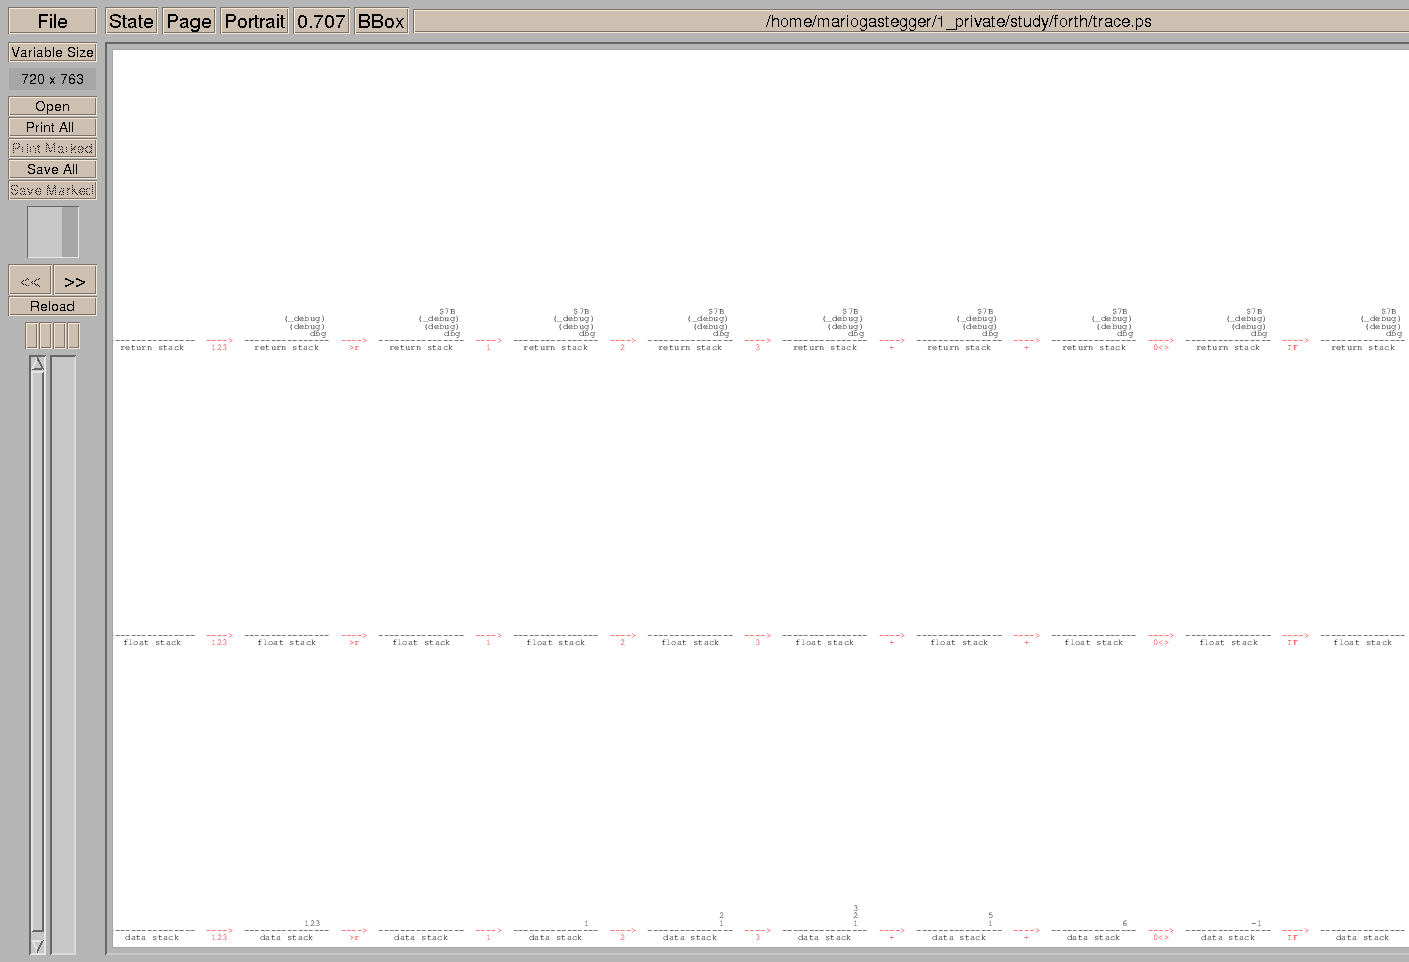
\includegraphics[scale=0.30]{graphics/traceps1.png}
    \caption{Output of trace.ps after typing \emph{dbg test}(part 1/2)}
    \label{fig:traceps1}
\end{figure}

\begin{figure}[p]
    \centering
    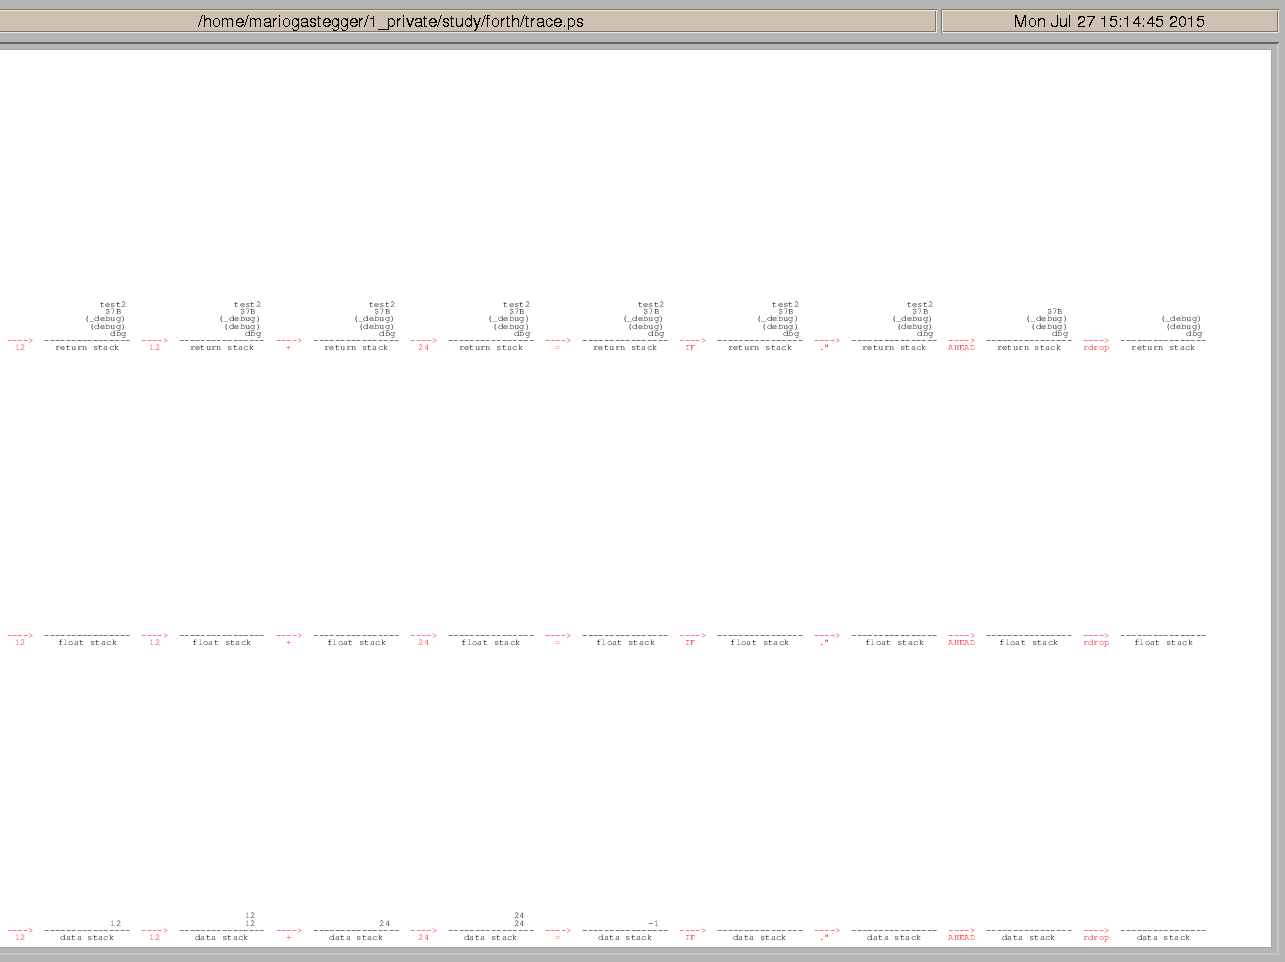
\includegraphics[scale=0.30]{graphics/traceps2.png}
    \caption{Output of trace.ps after typing \emph{dbg test}(part 2/2)}
    \label{fig:traceps2}
\end{figure}